\documentclass[12pt, a4paper]{article}

\usepackage{amsmath}
\usepackage{graphicx}
%\usepackage{setspace}
%\usepackage[cm]{fullpage}
\usepackage{a4wide}
\usepackage[colorlinks, breaklinks=true, bookmarks=true]{hyperref}

%\doublespacing

%\let\WriteBookmarks\relax

% functions and operations that shouldn't be in Italic font:
\newcommand{\sech}{\mathrm{sech}}
\newcommand{\Real}{\mathrm{Re}}
\newcommand{\Imag}{\mathrm{Im}}
\newcommand{\Tr}{\mathrm{Tr}}

% derivatives:

\newcommand{\deriv}[2]{\frac{d#1}{d#2}}
\newcommand{\nderiv}[3]{\frac{d^#3#1}{{d#2}^#3}}
\newcommand{\pderiv}[2]{\frac{\partial#1}{\partial#2}}
% 2'nd partial derivatives:
\newcommand{\spderiv}[2]{\frac{\partial^2#1}{{\partial#2}^2}}
\newcommand{\pderivdd}[3]{\frac{\partial^2#1}{\partial#2\partial#3}}
% functional derivatives:
\newcommand{\fnlderiv}[2]{\frac{\delta#1}{\delta#2}}
\newcommand{\fnlderivdd}[3]{\frac{\delta^2#1}{\delta#2\delta#3}}

% small matrix:
\newenvironment{bsmatrix}{\left[\begin{smallmatrix}}{\end{smallmatrix}\right]}

% big 0 in a matrix:
\newcommand{\BigFig}[1]{\parbox{12pt}{\Huge #1}}
\newcommand{\BigZero}{\BigFig{0}}
%\newcommand{\ket}[1]{\left|#1\right>}
\newcommand{\bra}[1]{\left<#1\right|}
% an eighenstate:
\newcommand{\eigs}[1]{\left|\varphi_{#1}\right>}
% brackets with operator:
\newcommand{\bracketsO}[3]{\left<#1 \left|#2 \right|#3 \right>}
% with a bigger |:
\newcommand{\bracketsObigm}[3]{\left<#1\! \bigm|\!#2 \!\bigm|\!#3 \right>}
% with the biggest |:
\newcommand{\bracketsObiggm}[3]{\left<#1\! \biggm|\!#2 \!\biggm|\!#3 \right>}
% brackets without operator:
\newcommand{\brackets}[2]{\left<#1 | #2\right>}
% with a bigger |:
\newcommand{\bracketsbigm}[2]{\left<#1 \bigm| #2\right>}
% with the biggest |:
\newcommand{\bracketsbiggm}[2]{\left<#1 \biggm| #2\right>}
% expectation value:
\newcommand{\exval}[1]{\left<#1 \right>}
% bold operator:
\newcommand{\operator}[1]{\mathbf{\hat#1}}
% commutation relation:
\newcommand{\commut}[2]{\left[#1, #2\right]}

\newcommand{\etal}{\textit{et al.}\ }
\newcommand{\ie}{i.\,e.\ }
\newcommand{\eg}{e.\,g.\ }

\begin{document}
\title{Two dimensional Poisson equation\\
Computational project No. 2}
\author{Ido Schaefer}
\date{\today}
\maketitle

\section{Iterative smoothing}

The iterative smoothing procedure is implemented in the function \texttt{smooth.m}.

The efficiency of the relaxation for several $\omega$ values is tested in the procedure \texttt{test\_smooth}. The root mean square of the residual:
\begin{equation}
	r_{rms} = \sqrt{\frac{\sum_{i,j}r_{i,j}^2}{(N-1)^2}} = \frac{|\mathbf{r}|}{(N-1)}
\end{equation}
is plotted Vs.\ the number of iterations ($N-1$ grid points in each dimension participate in the computational process). The procedure was employed for two $N$ values: $N=8$ and $N=16$. The results are shown in Figs.~\ref{fig:relaxw8}, \ref{fig:relaxw16}. It is shown that the relaxation is faster for the values $\omega=0.5$, $\omega=1$. The relaxation is faster for $N=8$, as expected.

\begin{figure}[htb]
	\centering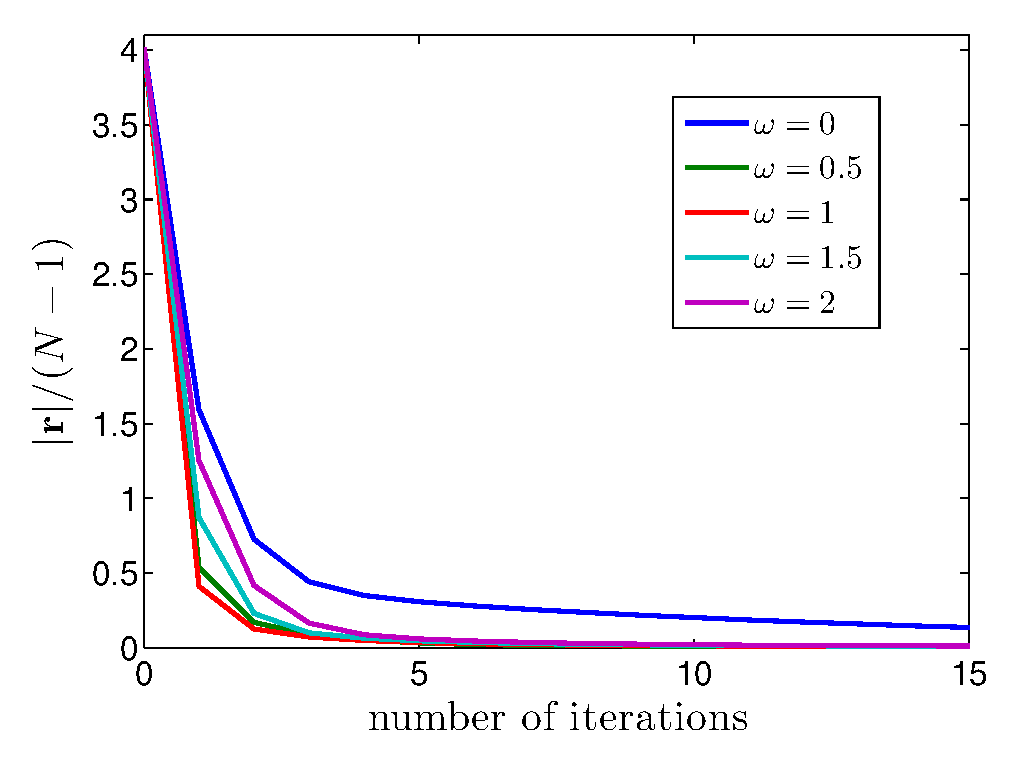
\includegraphics[width=3in]{relax_omega8}
	\caption{$r_{rms}$ Vs.\ the number of iterations for $N=8$, for several $\omega$ values.}\label{fig:relaxw8}
\end{figure}

\begin{figure}[htb]
	\centering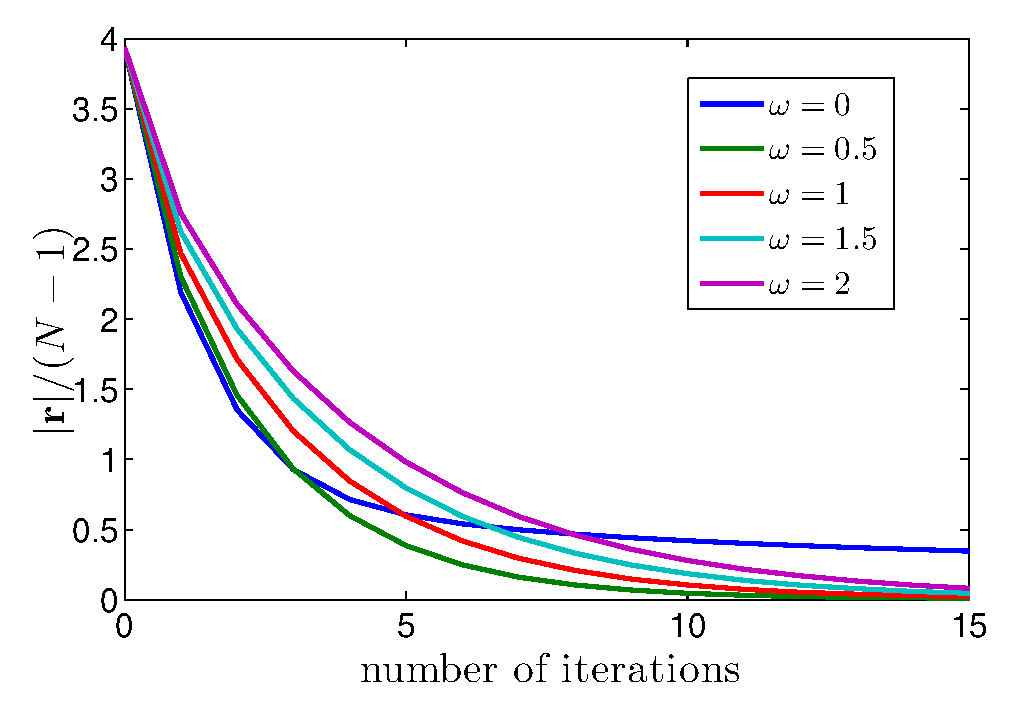
\includegraphics[width=3in]{relax_omega16}
	\caption{$r_{rms}$ Vs.\ the number of iterations for $N=16$, for several $\omega$ values.}\label{fig:relaxw16}
\end{figure}
 
The smoothing of the diagonal error function, $\epsilon(x, x) = \bar{\phi}(x, x) - \phi(x, x)$, during the iterative process is demonstrated by the procedure \texttt{smth\_diag}. The error function is plotted Vs.~$x$ for various iteration numbers in Fig.~\ref{fig:diag}. It is evident from the figure that the shape of $\epsilon(x,x)$ is getting smoother with the propagation of the iterative process.

\begin{figure}[htb]
	\centering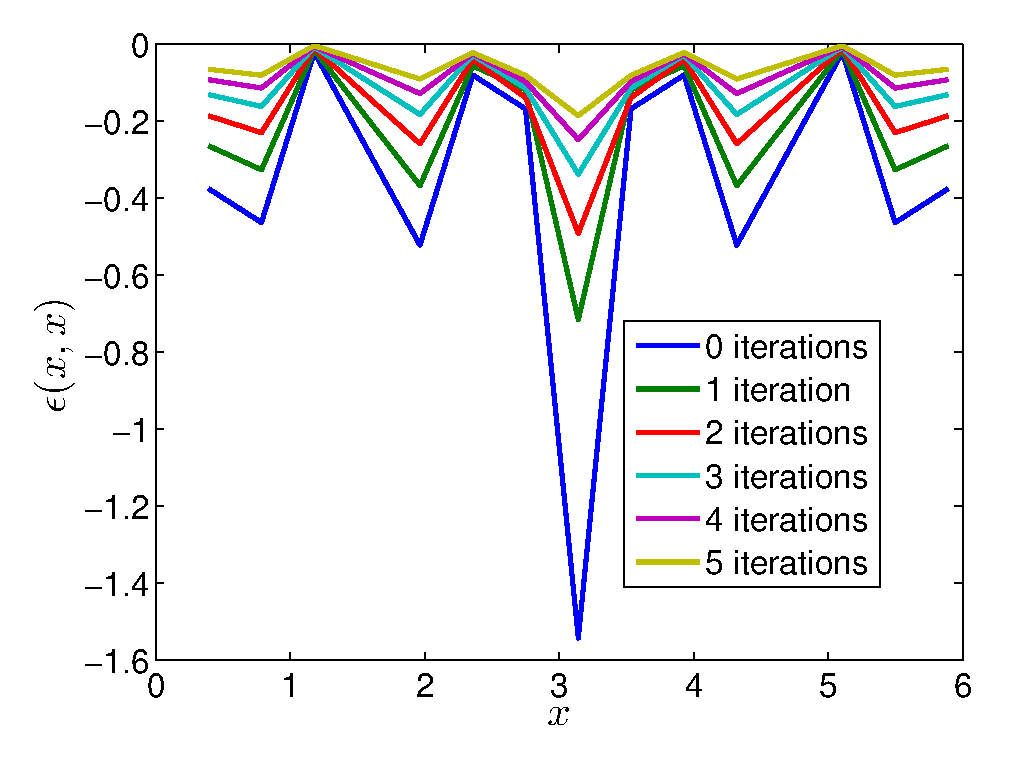
\includegraphics[width=3in]{smth_diag}
	\caption{$\epsilon(x, x)$ Vs.\ $x$ after various iteration numbers, from 0 to 5.}\label{fig:diag}
\end{figure}

\section{The multigrid method}

The multigrid method is implemented in the procedure \texttt{test\_multigrid.m}. The function \texttt{multigrid.m} performs a single V-cycle in a recursive process. In \texttt{test\_multigrid.m}, the multigrid method is tested for $N=16$, $\omega=0.5$, and for 10 smoothing iterations in each call to \texttt{smooth.m}.

The error decay is presented Figs.~\ref{fig:multr}, \ref{fig:multe}. We use two measures for the error --- the residual, and the relative deviation from the numeric solution (as solved by \texttt{MATLAB}), defined as:
\begin{equation}
	\epsilon_{rel} = \frac{|\phi - \bar\phi|}{|\phi|}
\end{equation}
In Fig.~\ref{fig:multr}, $\log_{10}(r_{rms})$ is plotted Vs.\ the number of V-cycles. In Fig.~\ref{fig:multe}, $\log_{10}(\epsilon_{rel})$ is plotted Vs.\ the number of V-cycles. The error decay rate shows exponential behaviour.

\begin{figure}[htb]
	\centering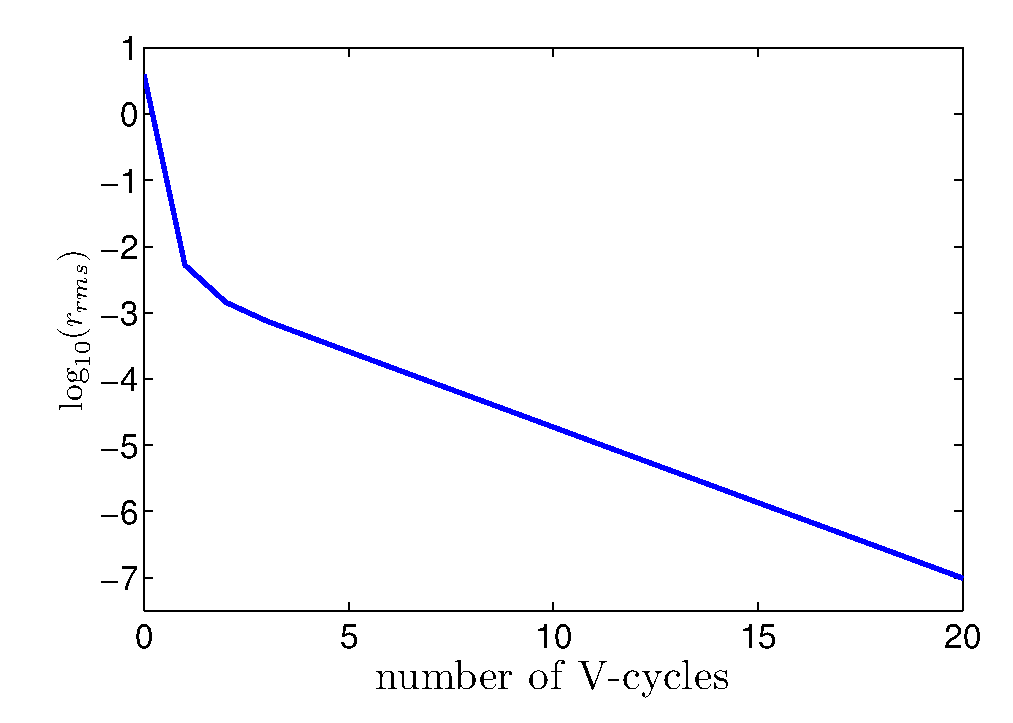
\includegraphics[width=3in]{multigridr}
	\caption{$\log_{10}(r_{rms})$ Vs.\ the number of V-cycles for $\omega=0.5$.}\label{fig:multr}
\end{figure}

\begin{figure}[htb]
	\centering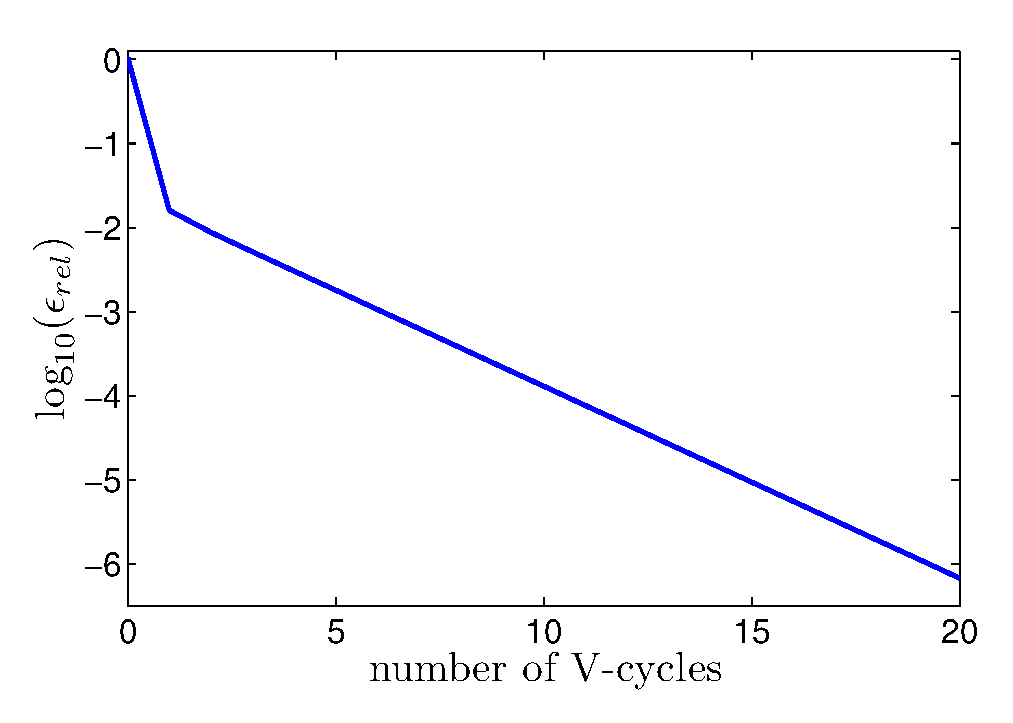
\includegraphics[width=3in]{multigrideps}
	\caption{$\log_{10}(\epsilon_{rel})$ Vs.\ the number of V-cycles for $\omega=0.5$.}\label{fig:multe}
\end{figure}

In the procedure \texttt{multg\_omega.m} the efficiency of the multigrid method is tested for several $\omega$ values. We use the same error measures as before. In Fig.~\ref{fig:multwr}, $\log_{10}(r_{rms})$ is plotted Vs.~$\omega$ for the sampling points:
\[
	\omega = 0,0.5,1,1.5,2
\]
In Fig.~\ref{fig:multweps}, $\log_{10}(\epsilon_{rel})$ is plotted Vs. $\omega$ in the same sampling points. It is shown that in the range of $\omega$ that has a relatively small reduction factor for high frequencies, the process is much more efficient.

\begin{figure}[htb]
	\centering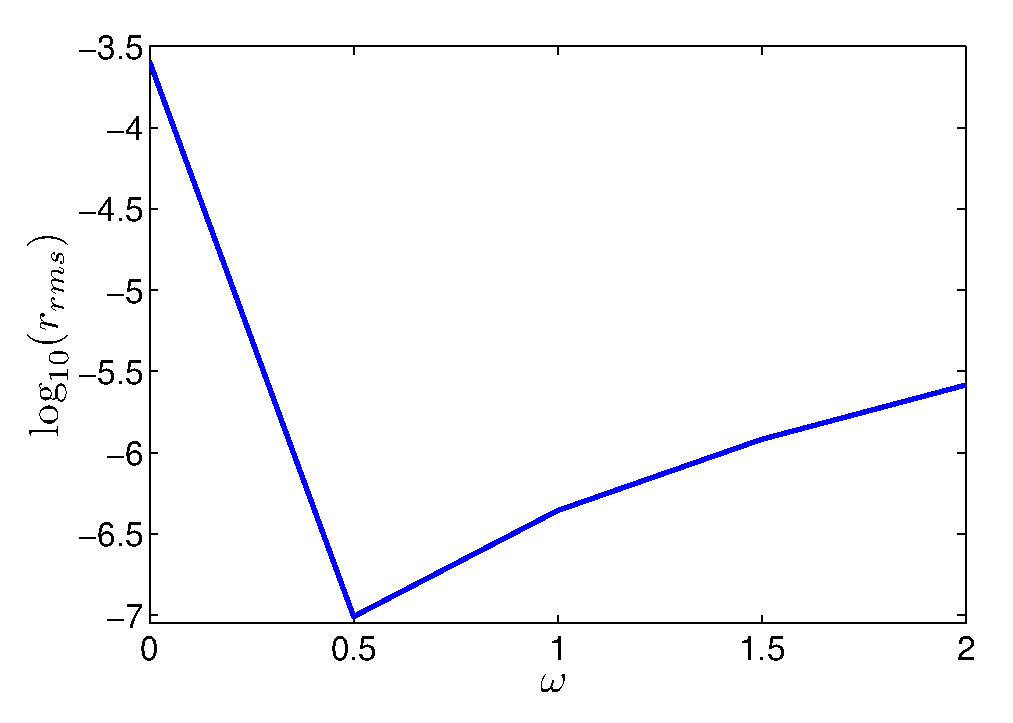
\includegraphics[width=3in]{multig_omega_r}
	\caption{$\log_{10}(r_{rms})$ after 20 V-cycles Vs.\ the $\omega$ value.}\label{fig:multwr}
\end{figure}

\begin{figure}[htb]
	\centering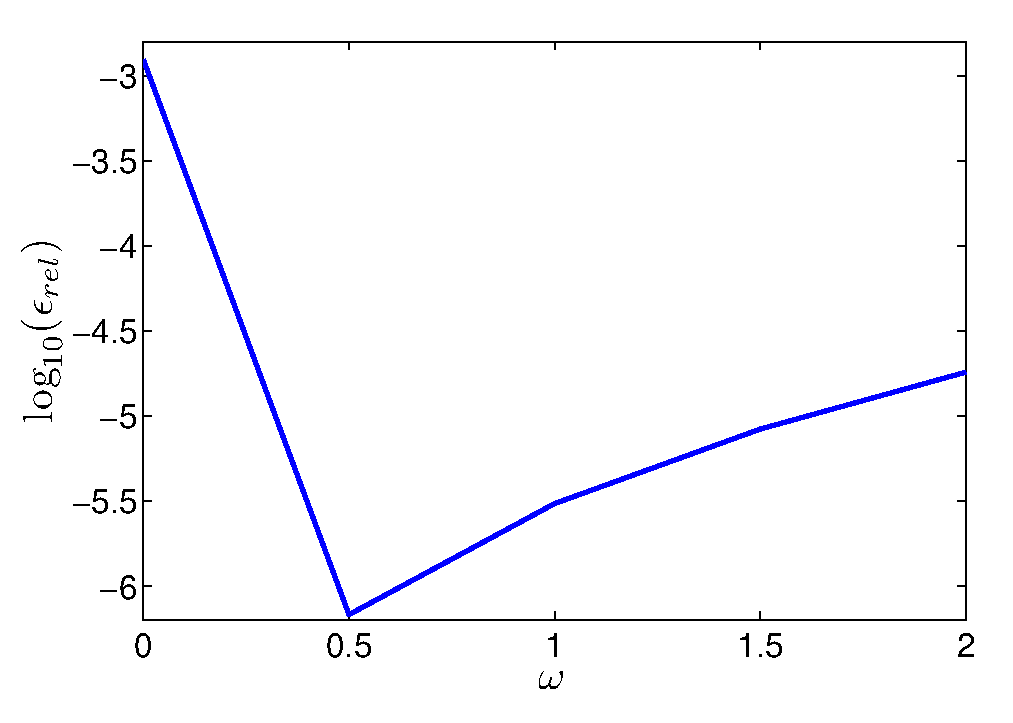
\includegraphics[width=3in]{multig_omega_eps}
	\caption{$\log_{10}(\epsilon_{rel})$ after 20 V-cycles Vs.\ the $\omega$ value.}\label{fig:multweps}
\end{figure}

\end{document}